\begin{table*}[t]
\centering
% \vspace{-1ex}
\renewcommand\arraystretch{0.93}
\caption{Main results (acc\%) on five in-distribution and six out-of-distribution VQA benchmarks. $^\dagger$ indicates results reported from the original papers. 
\emph{w/o Tools} excludes tool access from both training and inference stage; \emph{w/o Reasoning} removes RL training stage.
}
% \vspace{-1ex}
\resizebox{1.0\linewidth}{!}{ %
\begin{tabular}{l @{\hskip2.5pt} | c c c c c | c | c c c c c c  | c | c c }
\toprule
\textbf{Baselines ($\downarrow$)} &  \multicolumn{6}{c|}{\textbf{In-Distribution}} & \multicolumn{7}{c|}{\textbf{Out-of-Distribution}} & \textbf{All} \\
\cmidrule(lr){2-7} \cmidrule(lr){8-14} \cmidrule(lr){15-15}
\textbf{Datasets ($\rightarrow)$} & ChartQA & Geometry3K & GeoQA & UniGeo & MapQA & avg. & TABMWP & AI2D & PlotQA & CLEVR-Math & IconQA & MathVista  &  avg. &  avg.  \\
\midrule
\multicolumn{10}{l}{\textit{Commercial VLMs (For reference)}} \\
\midrule
%%%%%%%%%%%%%%%%%%%%%%%%%%%%%%%%%%%%%%
GPT-5 & 85.92 &	94.84 &	90.91 &	49.34 &	60.95 &	76.39 &	99.90 &	86.10 &	72.90 &	26.00 &	87.20 &	80.20 &	75.38 &	75.84 \\
GPT-5-mini & 82.80 &	91.01 &	88.01 &	46.02 &	61.35 &	73.84 &	98.57 &	85.85 &	70.95 &	27.15 &	87.73 & 79.30 &	74.93 &	74.43\\
GPT-o4-mini & 85.24 &	90.02 &	89.17 &	40.72 &	62.25 &	73.48 &	96.73 &	84.38 &	73.35 &	27.35 &	86.53 &	78.00 &	74.39 &	73.98 \\ 
GPT-o3 & 85.63 &	92.35 &	90.14 &	50.27 &	54.25 &	74.53 &	99.18 &	79.58 &	71.85 &	25.55 &	81.87 &	75.40 &	72.24 &	73.28 \\ 
Gemini-2.5-Pro & 83.64 & 94.34 & 86.85 & 60.34 & 64.20 &	77.87 &	99.90 &	90.28 &	77.40 &	25.70 &	96.93 & 82.00 &	78.70 &	78.33 \\
Gemini-2.5-Flash & 85.85 &	92.85 &	88.78 &	46.15 &	53.35 &	73.40 &	97.96 &	84.50 &	68.75 &	23.45 &	84.73 &	77.90 &	72.88 &	73.12 \\
Claude-4.5-Sonnet & 85.03 &	85.19 &	92.26 &	55.57 &	91.85 &	81.98 &	99.49 &	80.44 &	82.95 &	23.95 &	94.50 &	75.10 &	76.07	& 78.76 \\
\midrule
%%%%%%%%%%%%%%%%%%%%%%%%%%%%%%%%%%%%%%
\multicolumn{10}{l}{\textit{Base Size: < 7B parameters}} \\
\midrule
InternVL3-2B   & 24.08  &	40.26  &	40.21  &	21.88  &	16.35  &	28.56  &	82.41  &	63.59  &	38.94  &	17.90  &	60.13  &	32.70  &	49.28  &	39.86 \\
\rowcolor{magenta!12} \ours{} (InternVL3-2B) &  88.55 &	56.24 &	68.54 &	42.31 &	33.35 &	57.80 &	85.35 &	73.80 &	63.85 &	39.81 &	84.13 &	60.00 &	67.82 &	63.27 \\
\rowcolor{magenta!3} \quad w/o Tools  &	72.88  &	43.93  &	66.30  &	39.52  &	39.45  &	52.42  &	74.23  &	64.70  &	35.90  &	15.93  &	63.53  &	49.60  &	50.65  &	51.45 \\
\rowcolor{magenta!3} \quad w/o Reasoning & 43.76	& 43.43	& 54.93	& 23.47 &	25.05 &	38.13 &	85.27 &	51.29 &	30.85 &	21.24 &	68.53 &	28.30 & 47.58 &	43.28 	\\
Qwen2.5-VL-3B  & 40.08  &	38.09  &	34.40  &	19.00  &	18.00  &	29.91  &	82.05  &	64.69  &	40.02  &	23.07  &	41.00  &	34.60  &	47.57  &	39.51 \\
LLaVA‑OneVision-1.5-4B 	& 61.60	&	50.92	&	29.79	&	14.06	&	27.25	&	36.72	&	93.15	&	73.68	&	43.90	&	24.00	&	84.80	&	44.50	&	60.67	&	49.79\\
\midrule
%%%%%%%%%%%%%%%%%%%%%%%%%%%%%%%%%%%%%%
\multicolumn{10}{l}{\textit{Large Size: 7 - 13B parameters}}  \\
\midrule
Qwen2.5-VL-7B & 76.40 &	39.43 &	41.39 &	30.64 &	26.30 &	42.83 &	80.64 &	70.44 &	65.53 &	25.18 &	61.45 &	59.20 &	60.41 &	52.42 \\
\rowcolor{teal!15}  \ours{} (Qwen2.5-VL-7B) & 90.08 &	53.27 & 71.32 &	44.43 &	66.85 &	65.19 &	86.40 &	72.68 &	74.82 &	33.37 &	72.51 &	63.00 &	67.13 &	66.25  \\ 
\rowcolor{teal!4}  \quad w/o Tools & 83.32 &	48.92 &	68.11 &	33.42 &	51.35 &	57.02 &	64.13 &	56.09 &	76.45 &	26.92 &	68.58 &	56.10 &	58.05 &	57.58 \\	
\rowcolor{teal!4}  \quad w/o Reasoning & 79.68 &	47.92 &	58.61 &	34.88 &	26.70 &	49.56 &	82.11 &	72.09 &	66.90 &	17.93 &	82.87 &	42.50 &	60.73 &	55.65 \\					
VTool-R1-7B & 80.70$^\dagger$ & 62.06 &	65.18 &	33.29 &	19.65 &	52.18 &	64.21 &	79.34 &	48.85 &	19.70 &	75.67 &	36.60 &	54.06 &	53.20 \\
R1‑VL‑7B & 83.90$^\dagger$ &	58.90 &	62.09 &	37.93 &	23.87 &	57.34 &	92.64 &	76.51 &	48.50 &	18.00 &	87.27 &	63.50$^\dagger$ & 65.20 & 61.63 \\
R1‑Onevision‑7B  &59.92 &	55.79 &	57.47 &	28.30 &	33.20 &	46.94 &	84.19 &	61.75 &	35.40 &	19.30 &	79.30 &	64.10 &	57.34 &	52.61 \\	
Perception‑R1-7B & 	76.41 &	48.59 &	51.23 &	21.22 &	40.52 &	47.59 &	84.05 &	67.77 &	44.30 &	18.00 &	81.87 & 74.20$^\dagger$ &	61.70	& 55.29 \\	
InternVL3-8B   & 77.32 & 47.09 &	44.87 &	33.71 &	34.70 &	47.54 &	95.32 &	74.54 &	63.05 &	28.95 &	73.27 &	59.60 &	65.79 &	57.49 \\ 
\rowcolor{teal!15}  \ours{} (InternVL3-8B) &  91.92 &	61.27 &	76.41 &	49.67 &	68.45 &	69.54 &	96.52 &	79.86 &	66.38 &	38.20 &	91.09 &	62.80 &	72.48 &	71.14 \\ 
\rowcolor{teal!4}  \quad w/o Tool  & 84.24 &	51.47 &	73.10 &	34.70 &	53.50 &	59.40 &	94.68 &	75.37 &	60.25 &	29.24 &	80.93 &	62.80 &	67.21 &	63.66 \\
\rowcolor{teal!4}  \quad w/o Reasoning  & 68.56 & 35.64 &	55.90 &	27.06 &	26.45 &	42.72 &	92.34 &	50.45 &	38.70 &	28.18 &	80.07 &	29.10 &	53.14 &	48.40 \\ 
LLaVA‑OneVision-1.5-8B & 64.96 & 54.08 & 32.69 & 16.05 & 32.40 & 40.04 &	94.27 &	77.37 &	46.60 &	25.00 &	89.67 &	47.70 &	63.44 &	52.80 \\
\midrule
%%%%%%%%%%%%%%%%%%%%%%%%%%%%%%%%%%%%%%
\multicolumn{10}{l}{\textit{XL Size: > 13B parameters}}  \\
\midrule
InternVL3-14B &  87.30 &	68.89 &	75.05 &	41.78 &	50.77 &	64.76 &	97.71 &	75.40 &	74.12 &	32.83 &	81.47 &	71.67 &	72.20 &	68.82 \\
\rowcolor{blue!12}  \ours{} (InternVL3-14B) & 93.60 &	83.87 &	78.85 &	52.94 &	70.50 &	75.95 &	98.02 &	87.60 &	76.00 &	40.86 &	92.13 &	68.00 &	77.10 &	76.58   \\
Qwen2.5-VL-32B  & 87.30&	65.22&	50.29&	42.94&	89.20&	66.99&	94.79&	82.16&	71.17&	35.14&	92.60&	68.20&	74.01&	70.82	 \\
InternVL3-38B &  89.20 &	70.72 &	79.11 &	45.14 &	55.13 &	67.86 &	98.35 &	83.03 &	78.48 &	33.88 &	83.73 &	74.03 &	75.25 &	71.89 \\
InternVL3-78B  & 89.70&	78.76&	85.43&	53.40&	58.15&	73.09&	99.39&	85.85&	82.35&	25.15&	86.33&	78.80&	76.31& 74.85 \\
% \midrule
%%%%%%%%%%%%%%%%%%%%%%%%%%%%%%%%%%%%%%
% \multicolumn{10}{l}{\textit{Tool-Integrated Reasoning Baselines (For reference)}}  \\
% \midrule

% \midrule
% %%%%%%%%%%%%%%%%%%%%%%%%%%%%%%%%%%%%%%
% \multicolumn{10}{l}{\textit{Reasoning-Only Baselines (For reference)}}  \\
% \midrule

\bottomrule
\end{tabular}%
}
\label{tab:main_results}
\end{table*}

\section{实验}
\label{sec:exp}

\subsection{实验设置}
\noindent \textbf{评测数据集。}
遵循多项已有工作 \cite{liu2025visionreasoner,huang2025vision,han2025tiger,li2025self}，我们聚焦于\emph{推理密集型 VQA 任务}，评估 \env{} 在提升开源 VLM 工具集成推理能力方面的有效性。对\emph{分布内}评测，我们从 \env{} 的 13 个训练数据集中选取 5 个具有官方测试集划分的数据集；对\emph{分布外}泛化能力，我们进一步在 6 个未参与训练的基准上测试。更详细的数据集信息见附录 \ref{app:data}。

\noindent \textbf{基线。}
我们在 \env{} 上比较三类基线：(i) 基于 API 的闭源 VLM；(ii) 开源 VLM；(iii) 已经集成工具或推理能力的 VLM。除工具集成基线遵循其原有工具配置外，其他基线均在\emph{不开放工具访问}的设置下评测，因为如果没有充分智能体训练，直接给模型开放工具会显著损害性能（见表~\ref{tab:fig-tir}）。更多基线细节见附录~\ref{app:baseline}。

\noindent \textbf{实现细节。}
我们使用四个不同大小的骨干模型来实例化 \ours{}，包括 InternVL3-2B/8B/14B 和 Qwen2.5-VL-7B，并基于 Verl-Tool~\cite{jiang2025verltool} 实现训练。SFT 阶段训练 1 个 epoch，batch size 为 128，学习率为 $2\times10^{-6}$，上下文长度为 16,384 token。RL 阶段中，每张 GPU 的 micro-batch size 为 8，mini-batch size 为 128，每次更新使用 $G=8$ 条 rollout；正则系数设为 $\beta=10^{-3}$，最大响应长度设为 26,780 token，学习率为 $5\times10^{-7}$，总训练步数为 $E=300$。我们采用准确率（ACC）作为主要评测指标，所有实验均在 8 张 NVIDIA H200 GPU 上完成。Prompt 模板与更多实现细节见附录。

\subsection{主要实验结果}
表~\ref{tab:main_results} 给出了在 11 个视觉推理数据集上，使用 \env{} 训练得到的 \ours{} 与各类基线的对比结果。结果显示出三点关键信息。第一，\ours{} 在相近规模模型中表现非常强：尤其是 \ours{}-8B，相较于同尺寸基线提升了 9.51\% 到 18.72\%；即便\emph{不使用工具}，也能有 2.03\% 到 11.24\% 的提升。第二，RL 对提升 VLM 的 TIR 能力至关重要。单纯把工具暴露给 VLM 而不提供显式推理监督，会降低准确率；相比之下，RL 能带来显著收益，说明基础 checkpoint 并不天然具备稳健的 TIR 能力，而 RL 是解锁视觉推理中工具使用能力的关键。第三，\ours{} 具备很强的参数效率：\ours{}-2B 已能达到甚至超过若干 8B 基线的水平，而 \ours{}-8B 的表现则可与 38B 参数量级的基线相比肩。这些结果表明，\env{} 为工具集成智能体 RL 提供了可扩展训练场，使得开源 VLM 也能获得稳健的视觉推理能力。

\begin{figure*}[t]
    \centering
    \begin{subfigure}[t]{0.33\linewidth}
        \centering
        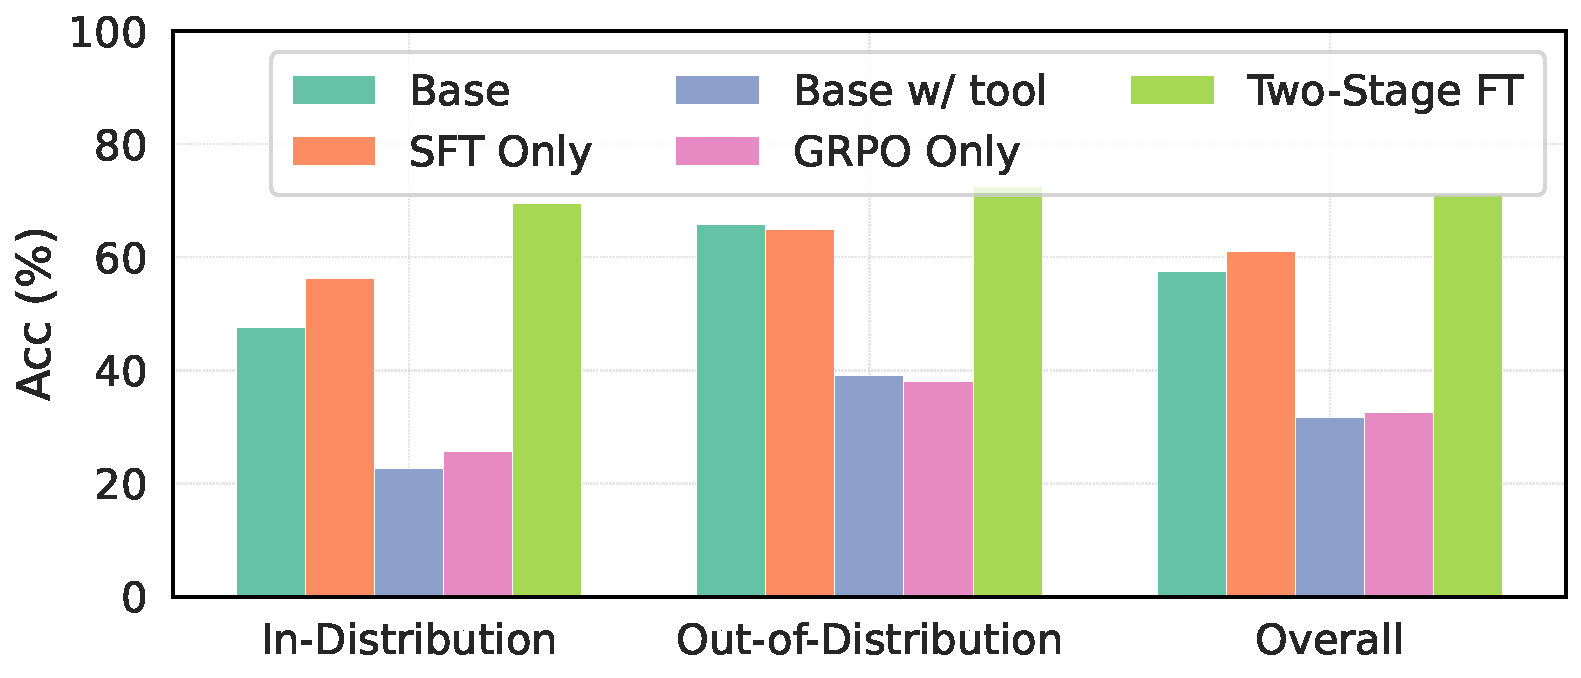
\includegraphics[width=\linewidth]{figure/effect-of-training-stage.pdf}
        \caption{训练阶段的影响}
        \label{fig:abl-training}
    \end{subfigure}
    \hfill
    \begin{subfigure}[t]{0.33\linewidth}
        \centering
        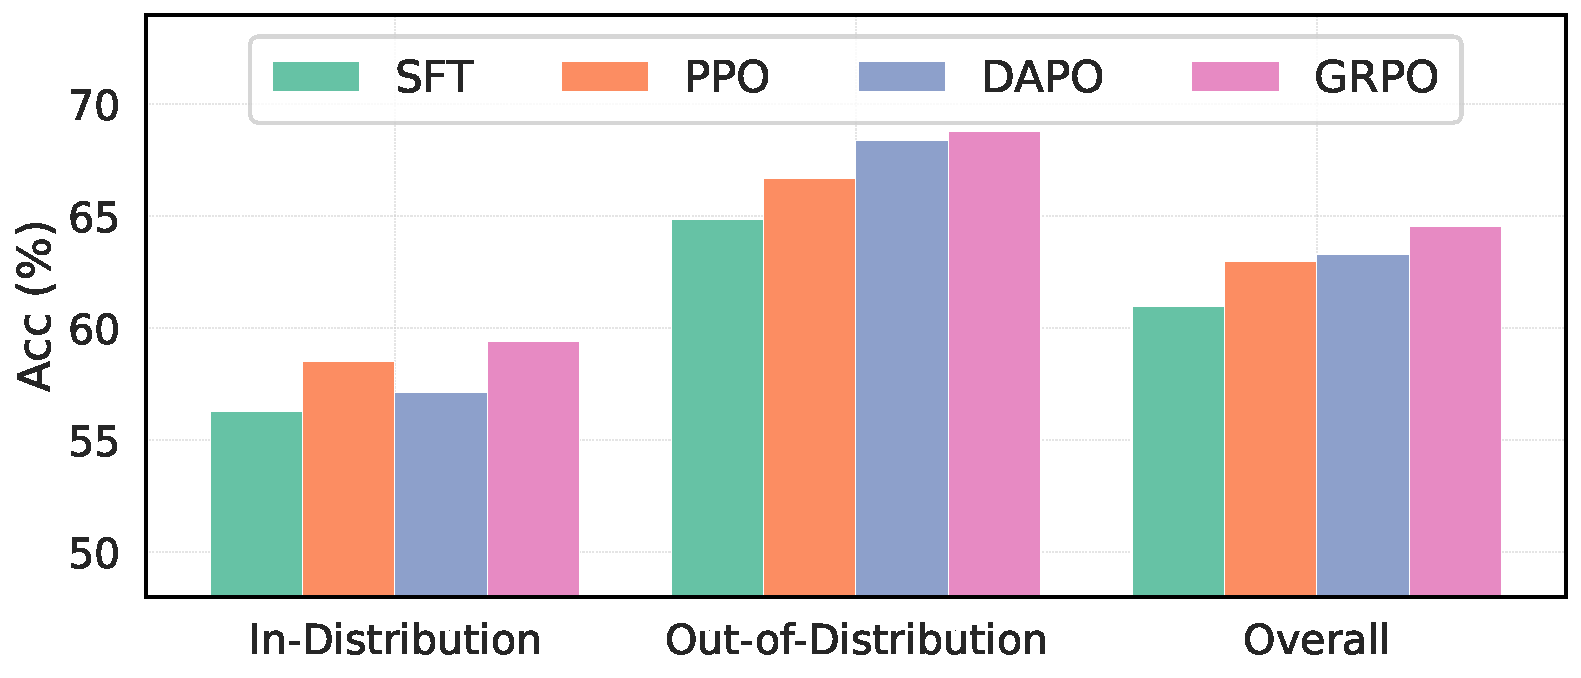
\includegraphics[width=\linewidth]{figure/effect-of-RL-method.pdf}
        \caption{RL 算法的影响（$E$=100）}
        \label{fig:abl-rl}
    \end{subfigure}
    \hfill
    \begin{subfigure}[t]{0.33\linewidth}
        \centering
        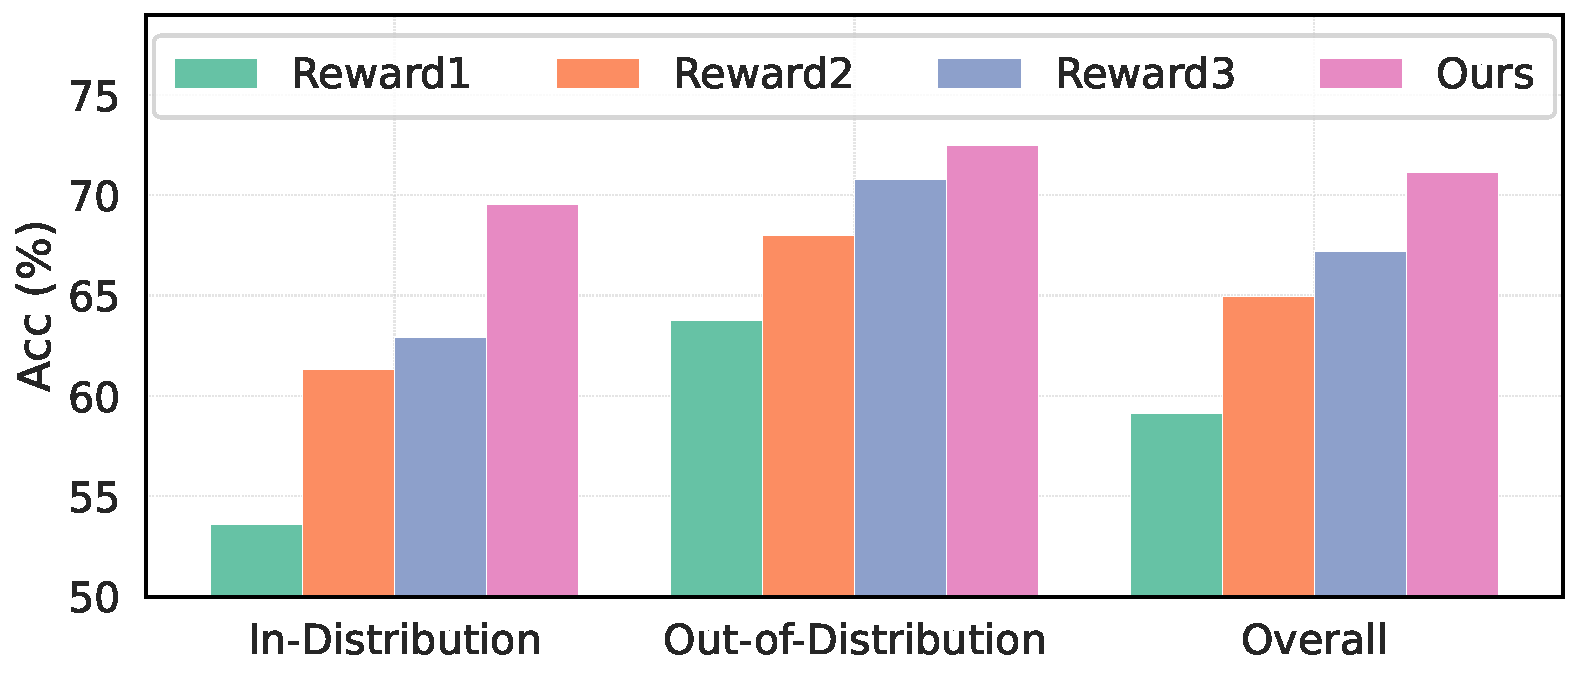
\includegraphics[width=\linewidth]{figure/effect-of-Reward.pdf}
        \caption{奖励设计的影响}
        \label{fig:abl-reward}
    \end{subfigure}
    \hfill
    \begin{subfigure}[t]{0.33\linewidth}
        \centering
        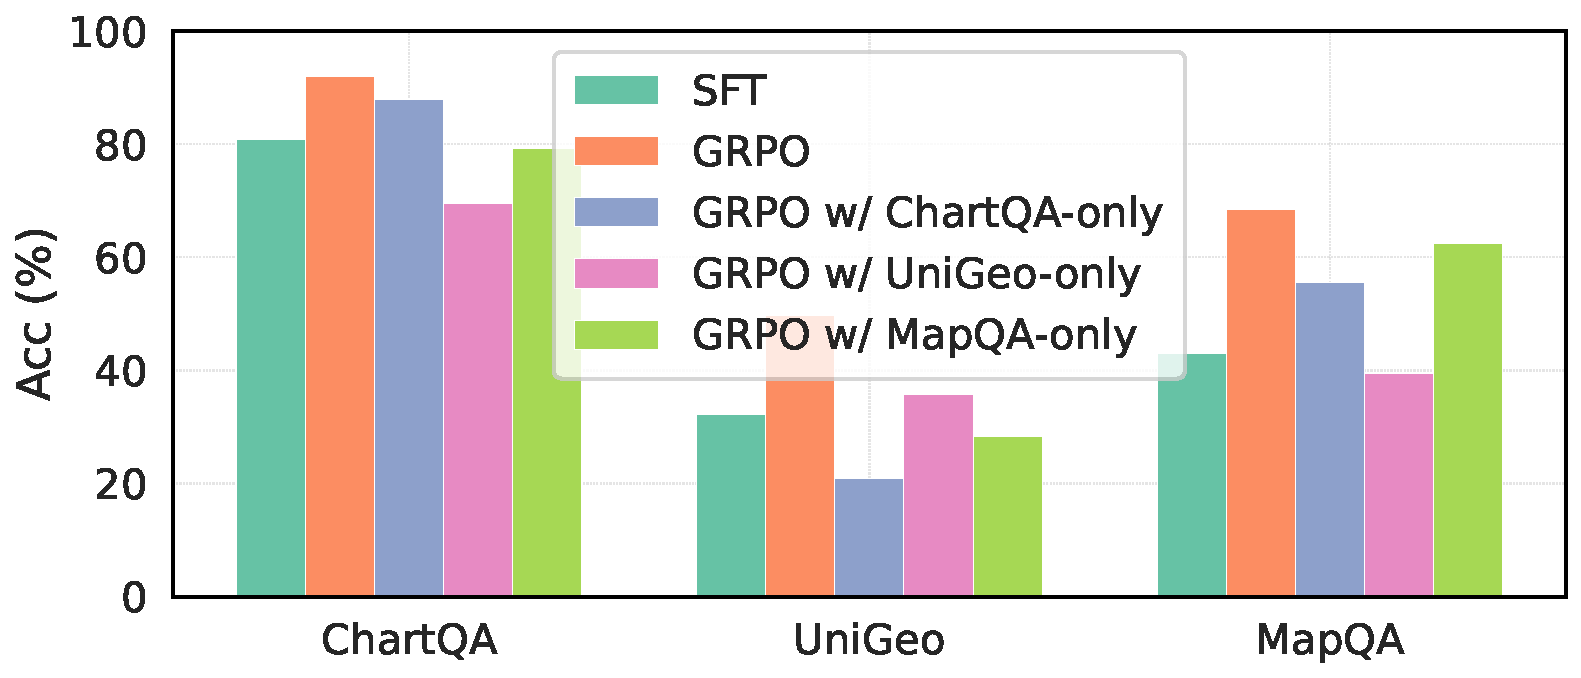
\includegraphics[width=\linewidth]{figure/effect-of-data-diversity.pdf}
        \caption{数据多样性的影响}
        \label{fig:adata-diversity}
    \end{subfigure}
    \hfill
    \begin{subfigure}[t]{0.33\linewidth}
        \centering
        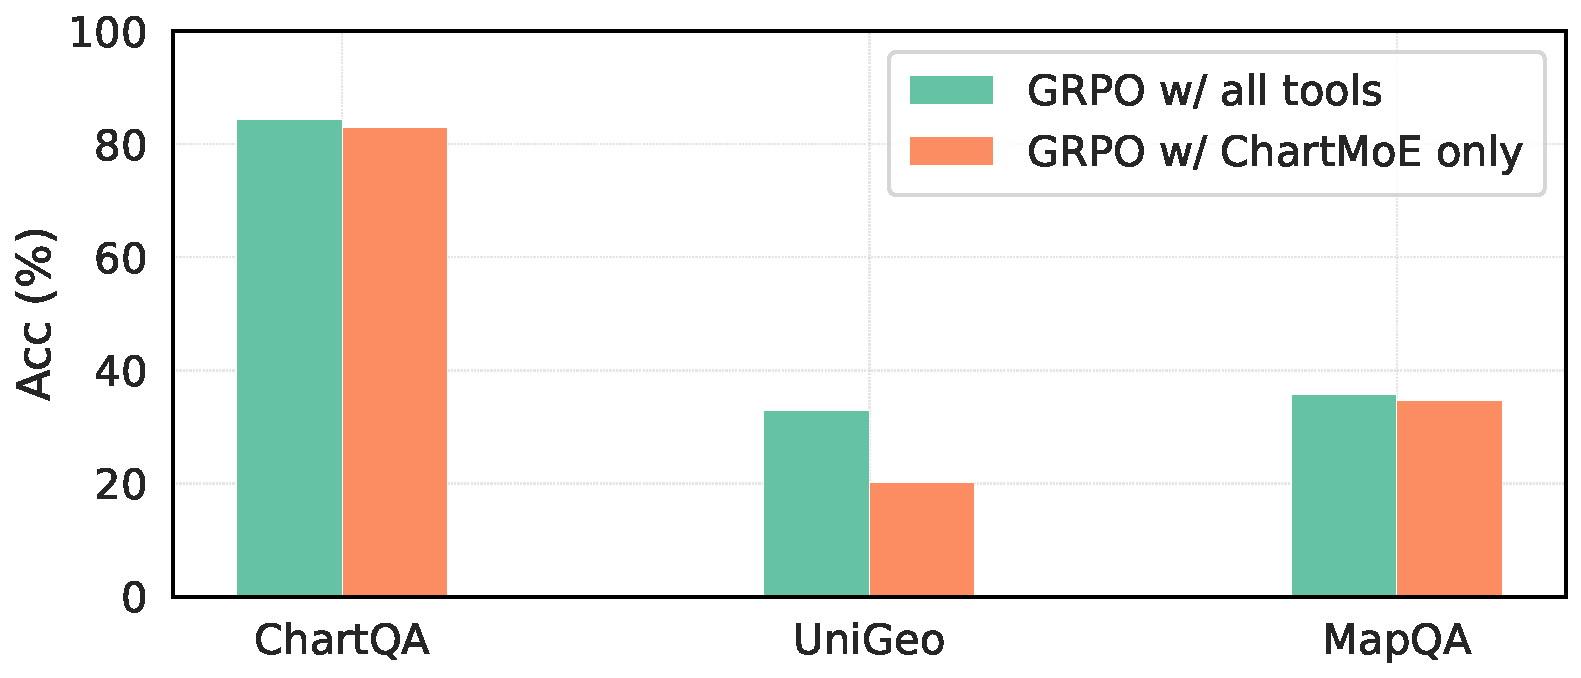
\includegraphics[width=\linewidth]{figure/effect-of-tool-diversity.pdf}
        \caption{工具多样性的影响（$E$=50）}
        \label{fig:tool-diversity}
    \end{subfigure}
    \hfill
    \begin{subfigure}[t]{0.33\linewidth}
        \centering
        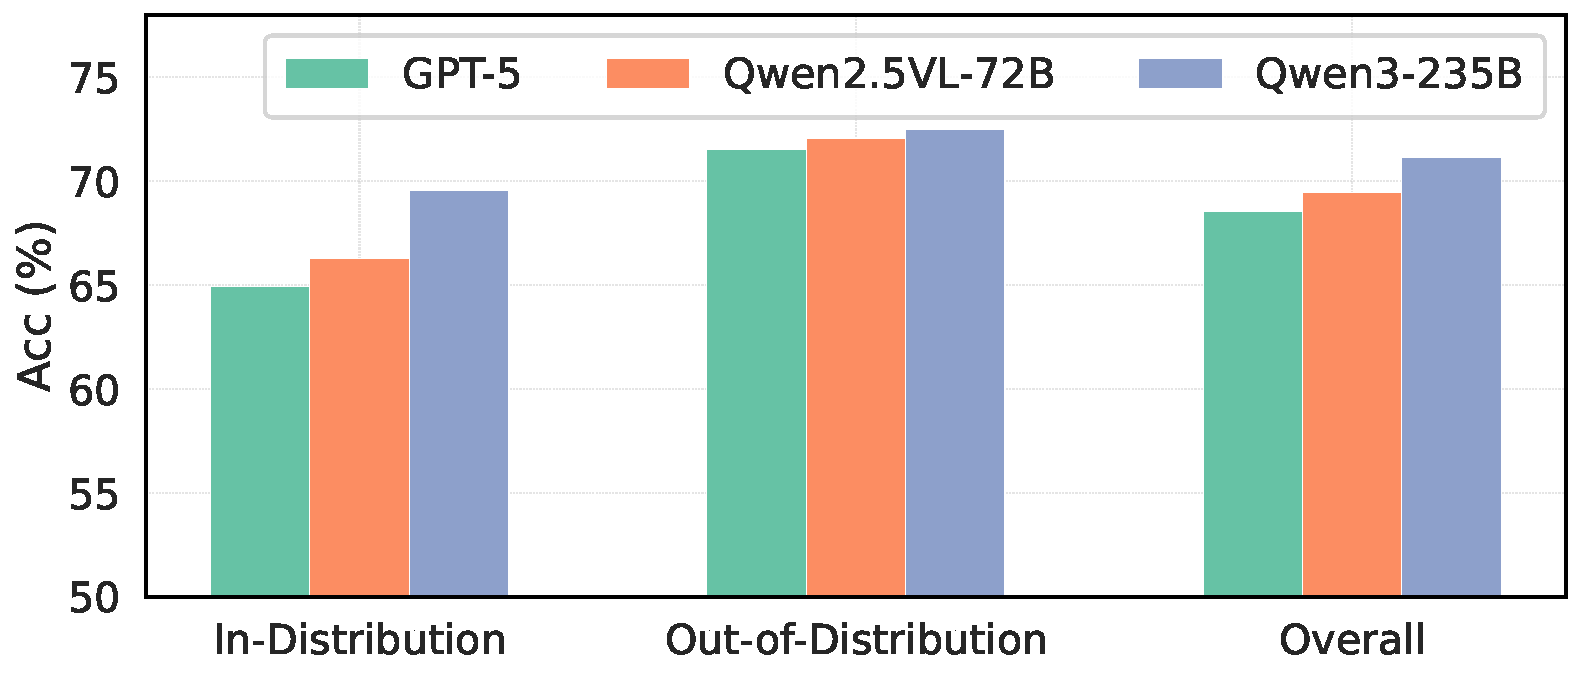
\includegraphics[width=\linewidth]{figure/effect-of-traj-quality.pdf}
        \caption{思维轨迹质量的影响}
        \label{fig:effect-of-traj-quality}
    \end{subfigure}
    \caption{以 InternVL3-8B 为骨干模型的消融实验与多样性分析。}
    \label{fig:ablation-study}
\end{figure*}

\begin{table*}[t]
\centering
\renewcommand\arraystretch{0.93}
% \vspace{-2ex}
\caption{Effect of reasoning and tool-use results without RL training. \emph{w/ Tools} refers to directly augmenting VLMs with tools significantly degrades accuracy; \emph{w/ Reasoning} refers to CoT reasoning without tools. \emph{w/ T\&R} refers to a different setting compared to TIR, only supplying \emph{tool‑selection prior knowledge} and interleaving reasoning with tool execution improve performance. }
\resizebox{1.0\linewidth}{!}{ %
\begin{tabular}{l @{\hskip2.5pt} | c c c c c | c | c c c c c c  | c | c c }
\toprule
\textbf{Baselines ($\downarrow$)} &  \multicolumn{6}{c|}{\textbf{In-Distribution}} & \multicolumn{7}{c|}{\textbf{Out-of-Distribution}} & \textbf{All} \\
\cmidrule(lr){2-7} \cmidrule(lr){8-14} \cmidrule(lr){15-15}
\textbf{Datasets ($\rightarrow)$} & ChartQA & Geometry3K & GeoQA & UniGeo & MapQA & avg. & TABMWP & AI2D & PlotQA & CLEVR-Math & IconQA & MathVista  &  avg. &  avg.  \\
\midrule
\rowcolor{gray!15}  GPT-5 & 85.92 &	94.84 &	90.91 &	49.34 &	60.95 &	76.39 &	99.90 &	86.10 &	72.90 &	26.00 &	87.20 &	80.20 &	75.38 &	75.84 \\
\quad w/ Tools & 58.60 & 74.04 & 65.00 & 28.78& 31.20 & 51.52 &69.83 & 65.07 & 46.75 & 18.96 & 60.53 & 42.60 & 50.62 & 51.03\\
\quad w/ Reasoning  & 85.68 & 91.01 & 86.27 & 51.25& 59.48 & 74.74 &99.81 & 83.03 & 84.73& 25.50 & 86.27 & 80.90 & 76.71 & 75.81\\
\quad w/ T\&R &  94.00 & 93.84 & 91.56 & 51.69 & 57.35& 77.69 & 98.92 & 84.62& 79.45 & 27.79& 91.07 & 57.80 & 73.28 & 75.28 \\
\midrule
\rowcolor{gray!15}  InternVL3-8B   & 77.32 & 47.09 &	44.87 &	33.71 &	34.70 &	47.54 &	95.32 &	74.54 &	63.05 &	28.95 &	73.27 &	59.60 &	65.79 &	57.49 \\ 
\quad w/ Tools & 25.44 &  17.06& 27.27 & 26.90& 16.22 & 22.58 &58.15 & 51.74 & 58.31 & 18.01 & 25.86 &  22.70& 39.13 & 31.61\\
\quad w/ Reasoning  & 81.28& 47.09 & 45.07 & 35.81&31.10 &  48.07& 94.38&76.51 & 65.85& 24.15 &75.53  &60.70  & 66.19 &57.95\\
\quad w/ T\&R & 68.56 & 35.64 & 55.90& 27.06 & 26.45&42.72 & 92.34 & 50.45& 38.70& 28.18& 80.07& 29.10& 53.14 &48.40 \\
% \midrule
% \rowcolor{gray!15}  InternVL3-2B   & 24.08  &	40.26  &	40.21  &	21.88  &	16.35  &	28.56  &	82.41  &	63.59  &	38.94  &	17.90  &	60.13  &	32.70  &	49.28  &	39.86 \\
% \quad w/ Tools & 19.20& 7.65 & 23.02 & 19.23& 8.45 & 15.51 & 34.00& 17.72& 29.05 & 1.81 & 25.40 & 21.70 & 21.61 & 18.84\\
% \quad w/ Reasoning  & 69.28 & 43.59 &42.82  &24.14 & 20.10& 39.99 & 87.88& 63.71 &43.25 &19.35 & 68.19 & 52.00 &55.73  & 48.57\\
% \quad w/ T\&R & 43.76  &43.43 &54.93  & 23.47 & 25.05& 38.13 & 85.27 &51.29 & 30.85 & 21.24& 68.53 & 28.30 & 47.59 & 43.28 \\
\bottomrule
\end{tabular}%
% \vspace{-2ex}
}
\label{tab:fig-tir}
\end{table*}

\subsection{\ours{} 的消融实验}
\noindent \textbf{工具集成推理的作用。}
表~\ref{tab:main_results} 还专门拆分了\emph{推理}与\emph{工具使用}的作用，分别报告了三种变体：(1) \emph{w/o Tools}，保留推理但禁用工具访问；(2) \emph{w/o Reasoning}，提供工具与工具选择先验，但不强化推理；(3) 同时交错推理和工具使用的完整 \ours{}。结果表明，仅加强推理或仅开放工具虽然偶尔能带来收益，但都明显不如完整 \ours{}。两个结论尤为明显：其一，若缺乏足够推理能力来导航动作空间，单纯开放工具反而可能有害；其二，最优问题求解方式来自“由推理引导工具调用”的交错闭环，而不是单独依赖其中任一能力。

\noindent \textbf{奖励设计的作用。}
图~\ref{fig:abl-reward} 比较了多种奖励设计，包括稠密奖励、稀疏奖励、难度自适应奖励以及本文设计。相比之下，我们的奖励把\emph{可验证、低噪声的二值终局信号}与基于组归一化优势的\emph{难度自适应缩放}结合起来，因此能在避免过拟合简单样本或利用中间信号漏洞的同时，实现更好的准确率。

\noindent \textbf{原始 VLM 中工具和推理的作用。}
表~\ref{tab:fig-tir} 总结了在开源和闭源原始 VLM 上，工具与推理各自带来的影响。直接给 VLM 开放工具通常会显著降低准确率，而仅靠内在 CoT 推理在复杂 VQA 上带来的提升也很有限。提供\emph{工具选择先验}能够改善表现，但其收益在商业 VLM 上高度任务依赖，小型开源 VLM 仍然困难重重。这些现象共同说明，为 VLM 赋予稳健、可泛化且适配多种视觉推理场景的工具使用能力既重要又不容易。

\begin{figure*}[t]
    \centering
    \begin{minipage}[t]{0.72\linewidth}
        \centering
        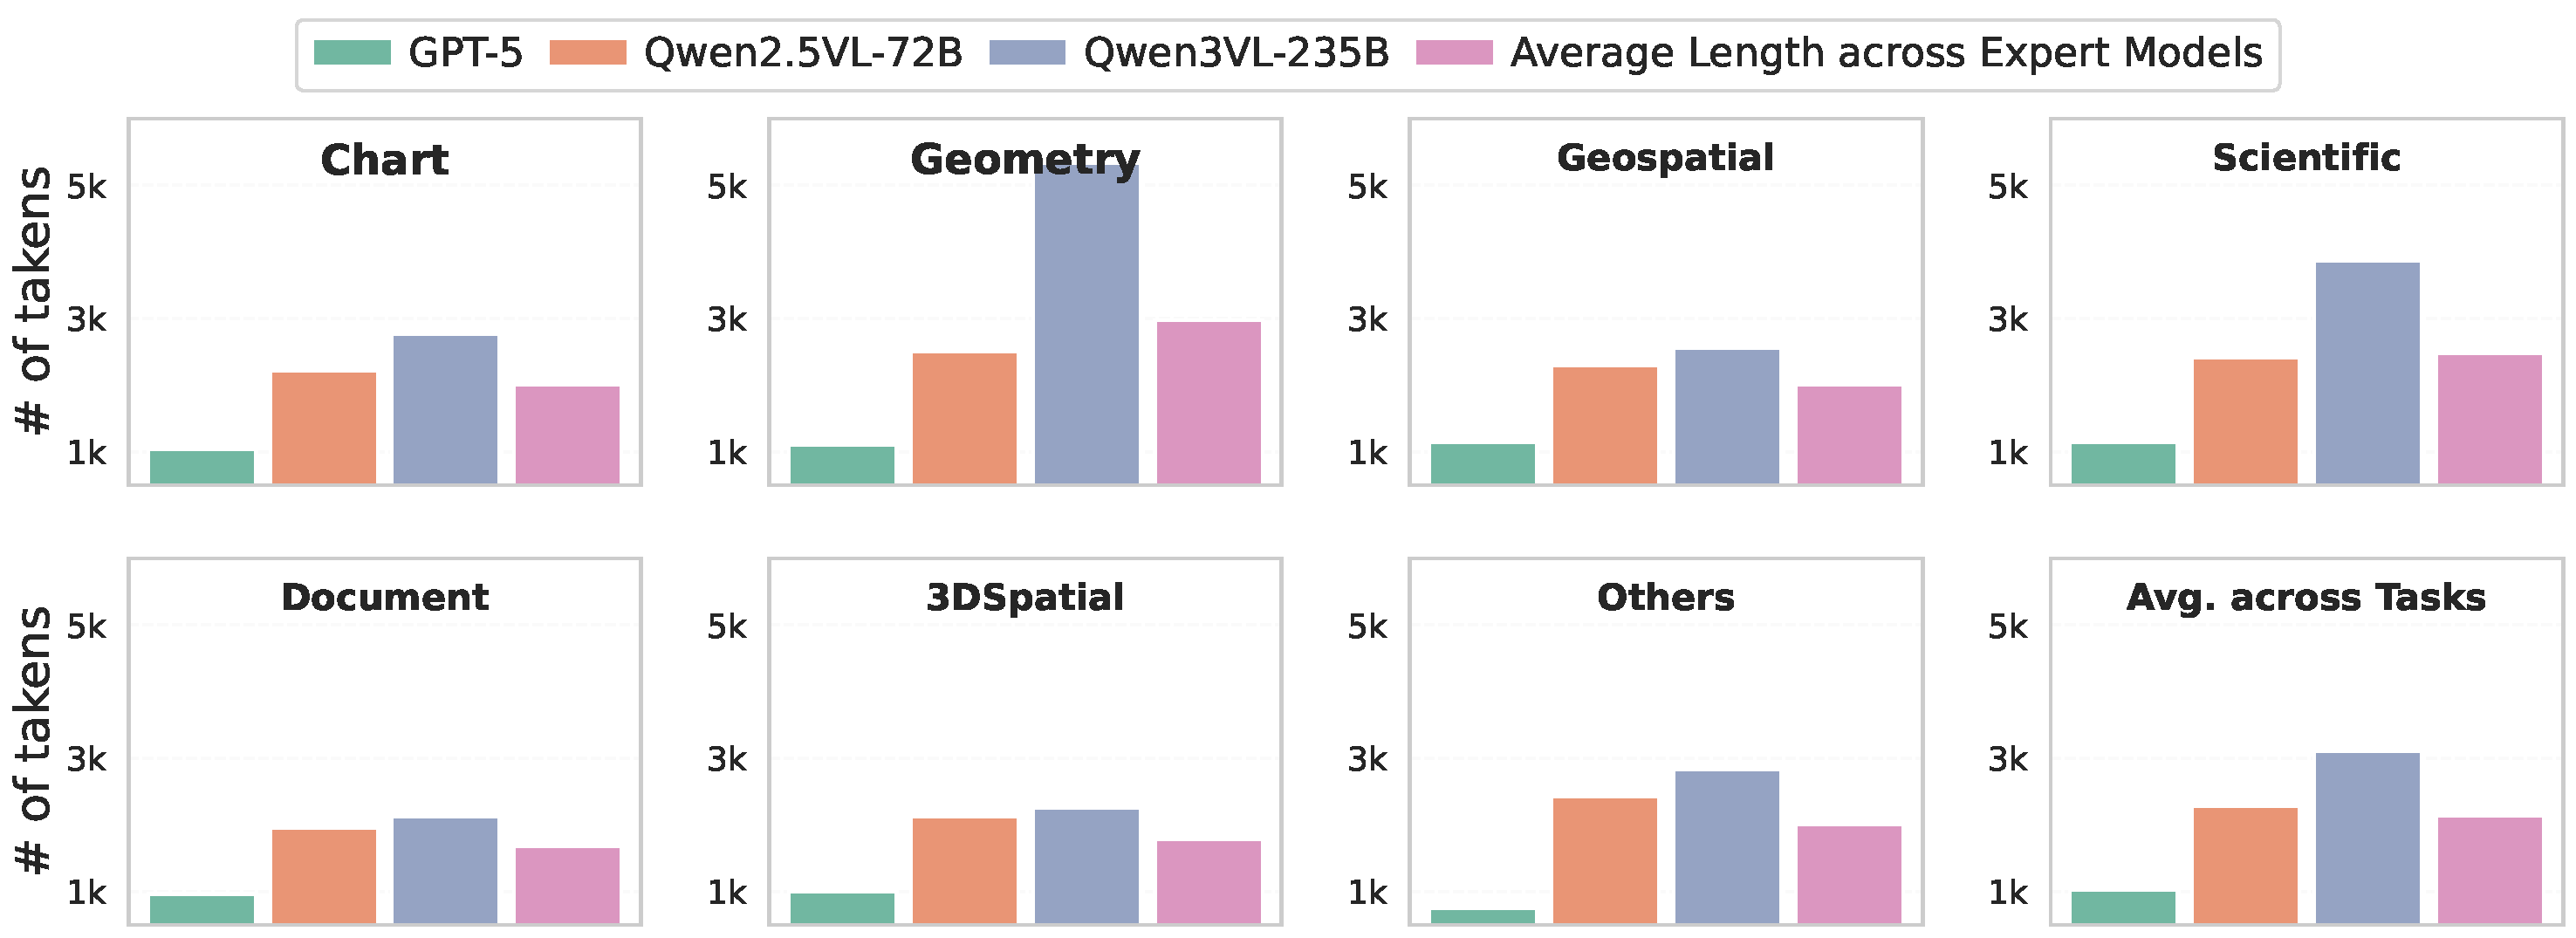
\includegraphics[width=\linewidth]{figure/traj-quality.pdf}
        \caption{不同长度专家思维轨迹的质量。}
        \label{fig:traj-quality}
    \end{minipage}
    \hfill
    \begin{minipage}[t]{0.27\linewidth}
        \centering
        
\includegraphics[width=\linewidth]{figure/error_analysis.pdf}
        \caption{错误分析。}
        \label{fig:error-transfer}
    \end{minipage}
\end{figure*}

\begin{figure}[t]
    \centering
    \begin{subfigure}[t]{0.49\linewidth}
        \centering
        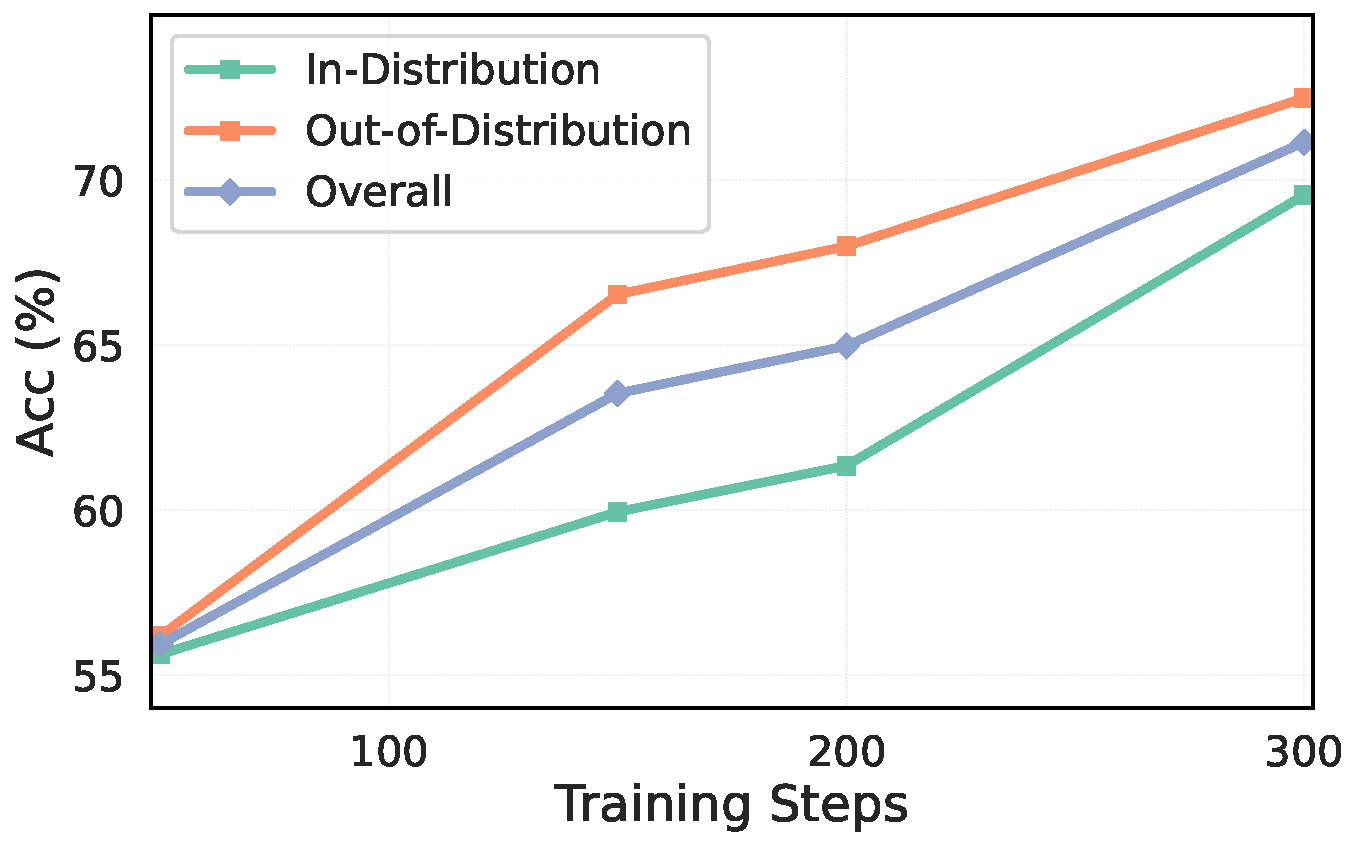
\includegraphics[width=\linewidth]{figure/epoch_plot.pdf}
        \caption{训练扩展}
        \label{fig:train-scale}
    \end{subfigure}
    \hfill
    \begin{subfigure}[t]{0.49\linewidth}
        \centering
    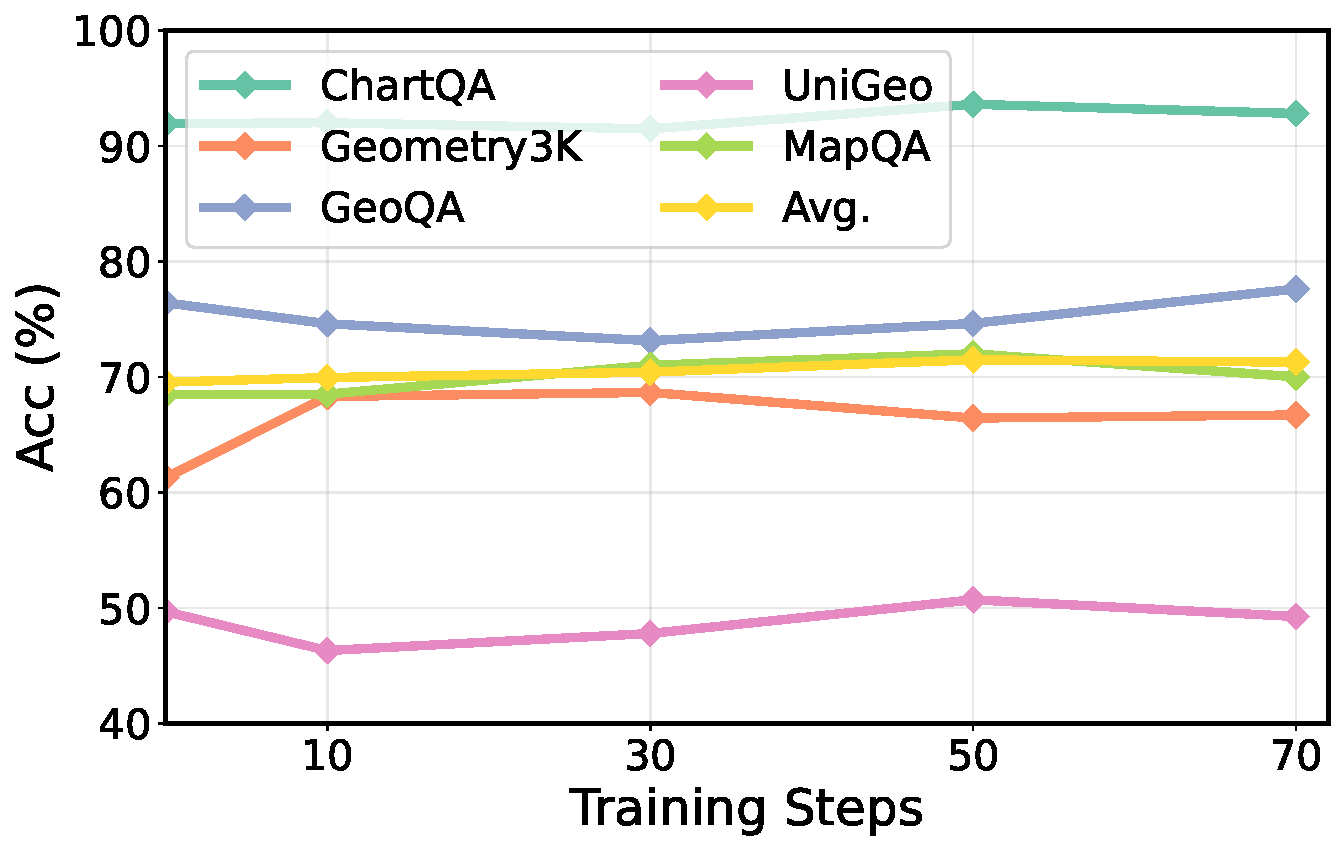
\includegraphics[width=\linewidth]{figure/tailpatch.pdf}
    \caption{Tailpatch}
    \label{fig:tailpatch}
    \end{subfigure}
    \caption{从易到难的训练扩展。}
    \label{fig:scale}
\end{figure}

\subsection{\env{} 的更多分析}
\noindent \textbf{数据多样性：数据混合的作用。}
图~\ref{fig:adata-diversity} 研究了 RL 期间任务组成如何影响 TIR。单任务训练的跨任务迁移能力较弱，特别是在不同领域之间；而多任务训练则更稳定地提升泛化能力，说明在训练期间接触多样化任务混合，对学习可迁移的 TIR 策略十分关键。

\noindent \textbf{工具多样性：工具混合的作用。}
图~\ref{fig:tool-diversity} 以 ChartMoE 为例分析工具组成对 TIR 的影响。只在单一工具类别上训练，会导致策略在该类任务上有效，但向其他工具结构差异较大的任务迁移能力有限。与数据混合类似，接触更多样的工具模式与参数格式，可以显著缓解过度专门化，并拓宽学到的动作策略。

\noindent \textbf{推理轨迹质量。}
我们用 token 长度作为一个简单代理，评估不同专家轨迹（GPT-5、Qwen2.5VL-72B、Qwen3VL-235B）的质量，结果见图~\ref{fig:traj-quality}。如预期，更长的轨迹在 SFT 预热阶段能建立更强的行为先验，因此在后续 RL 中带来更高性能（图~\ref{fig:effect-of-traj-quality}）。需要注意的是，商业 API 如 GPT‑5 往往不会公开全部中间推理，因此生成轨迹明显更短，在相同训练配方下对智能体 RL 的增益也更弱。

\noindent \textbf{Tail-Patch 课程学习。}
为了突破性能平台期，我们采用从易到难的课程策略，通过 \emph{tail-patch} 持续加入更困难的样本。我们把前一 checkpoint 的 rollout 通过率作为动态难度信号，筛出通过率落在 $[0.125, 0.375]$ 的“难但可学”样本。只在这一高难度子集上继续 RL，能够把性能从 69.54\% 进一步提升到 71.27\%（图~\ref{fig:scale}）。这表明，一个通用原则是把优化预算集中在模型“能力边界”附近的样本上。

\subsection{错误分析与案例研究}
\noindent \textbf{错误分析。}
我们在 InternVL3-8B 经 \env{} 训练前后，对表~\ref{tab:error-def} 中相同的 500 个样本重新做错误模式分析。结果显示，\env{} 中的智能体训练显著减少了基础模型中常见的大部分工具调用错误与推理错误。

\begin{figure}[t]
    \centering
    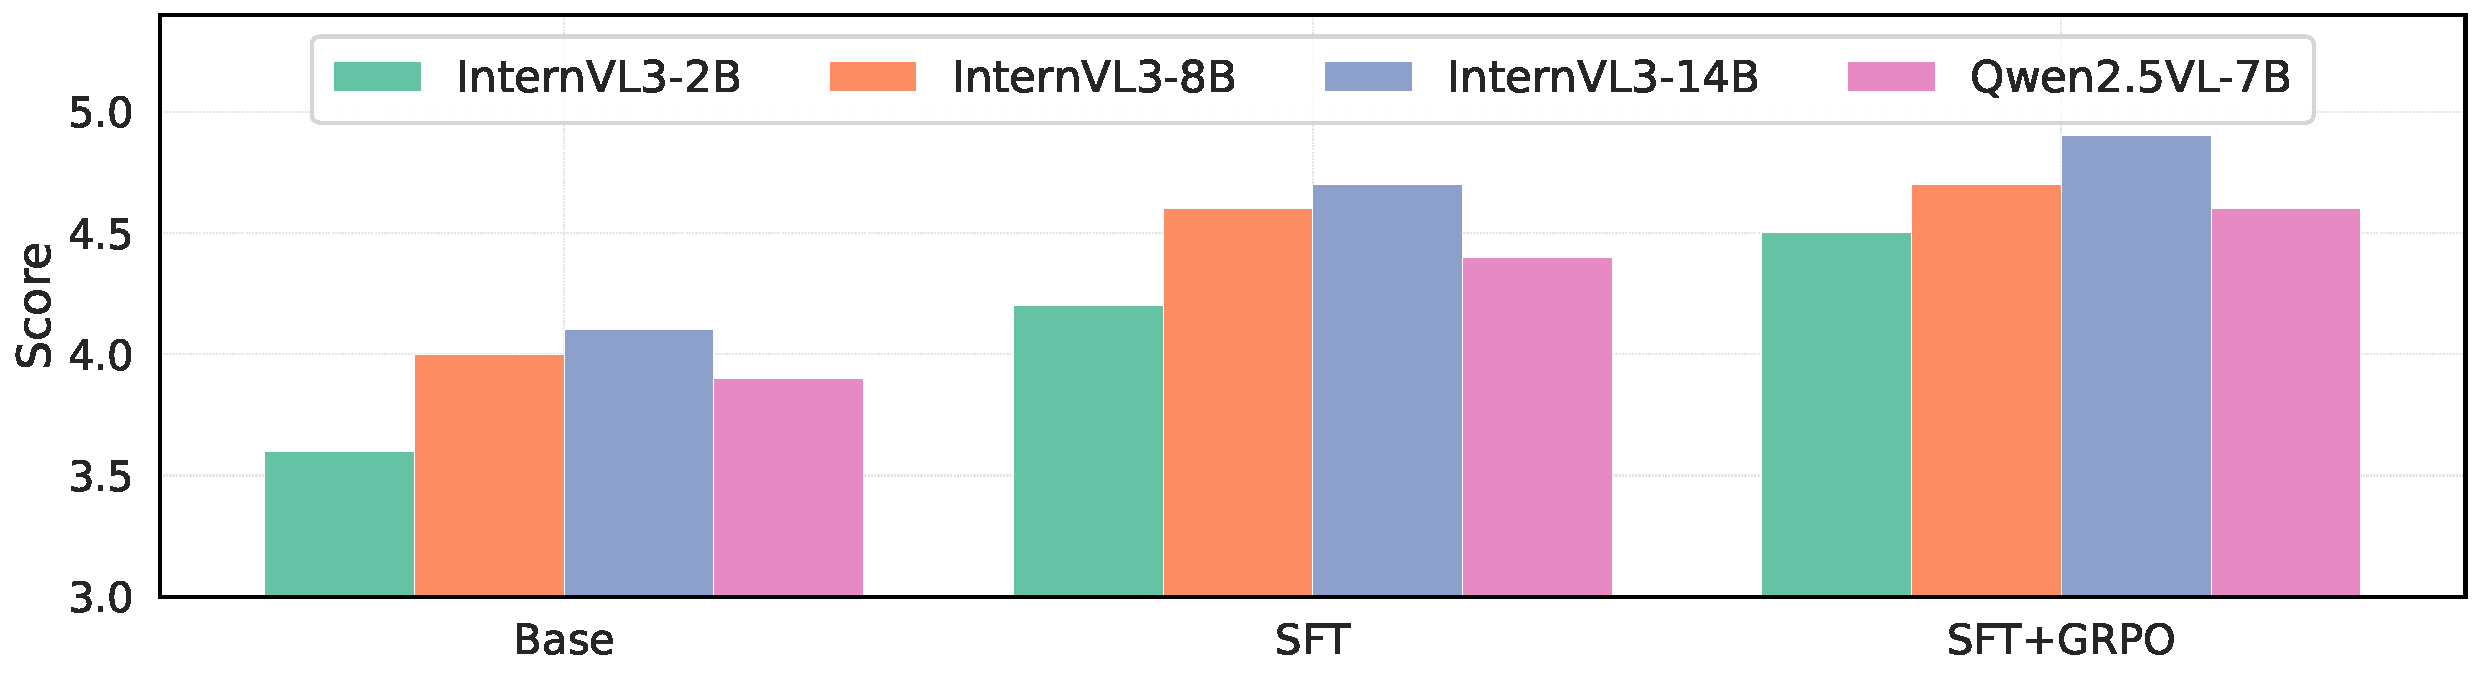
\includegraphics[width=\linewidth]{figure/human-study.pdf}
    \caption{关于轨迹质量的人类评测。}
    \label{fig:human-study}
\end{figure}

\noindent \textbf{轨迹质量的人类评测。}
由于 TIR 轨迹是 \env{} 的关键组成部分，我们还对生成出的交错工具使用与推理步骤质量进行了人工评估。图~\ref{fig:human-study} 报告了每个数据集随机抽取 40 条解题轨迹后的平均人工评分（1–5 分）。结果表明，两阶段训练都显著改善了不同任务和不同模型规模下的 TIR 质量。

\begin{table*}[t]
\centering
\renewcommand\arraystretch{0.95}
\caption{Case studies on geometric reasoning tasks with \ours-8B trained in \env{}.}
\resizebox{\linewidth}{!}{
    \begin{tabular}{p{1.8cm}p{21cm}}
    % \begin{tabular}{p{2cm}p{18cm}}
       \toprule
       \multicolumn{2}{l}{\textbf{Case Study 1}: Find m $\angle$ R. \textbf{Answer: A}: 58} \\
       % \midrule
        % \bf Q / A & who hosted and won the inagural world cup / Uruguay  \\
        \midrule
        \bf \multirow{6}{*}{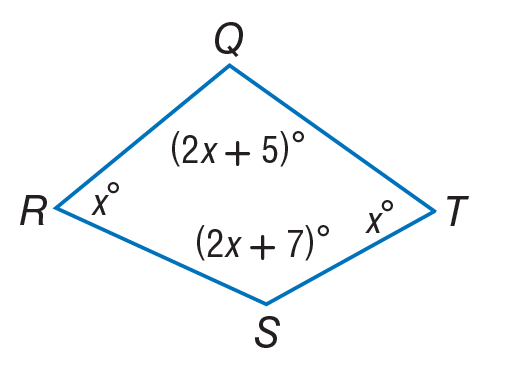
\includegraphics[width=\linewidth]{figure/casestudy/2489_img_diagram.png}} & \textbf{InternVL3-8B-Tool}: \textcolor{blue}{<tool\_call>}\{"tool": "multimath", "task": "solve\_the\_problem", "arguments": \{"image\_url": <image\_url>, "data": \{\textcolor{red}{"image/png": base64, iVBORw0KGgoAAAANSUhEUgAAAOAAAAHCAIAAADYXJpAAAAA3NCSV $\cdots$ (including long base64 image data)}\}\}\textcolor{blue}{</tool\_call>} \hfill \colorbox{red!15}{\textbf{Tool Call Error}: \emph{Invalid Arguments}. (\ding{56})} \\
        & \textbf{\ours}: \textcolor{blue}{<tool\_call>}\{"tool": "gllava", "task": "solve", "arguments": "Find m $\angle R$ from the diagram: a diamond-shaped quadrilateral with vertices R (left), Q (top), T (right), S (bottom). Angles labeled: at $R = x^\circ$, at $T = x^\circ$, at $Q = (2x+5)^\circ$, at $S = (2x+7)^\circ$."\}.\textcolor{blue}{</tool\_call>} \hfill \colorbox{green!15}{\textbf{Tool Call}: \emph{Correct} (\ding{51})} \\
        \midrule
        \multicolumn{2}{p{23cm}}{\textbf{Case Study 2}: As shown in the figure, in $\odot O$, $AB$ is a diameter and $CD$ is a chord. $AB \perp CD$, with the foot of the perpendicular at point $E$. Connect $CO$ and $AD$. If $\angle BOC = 30^\circ$, then the degree measure of $\angle BAD$ is ( ). \textbf{Answer: 15$^\circ$}} \\
        \midrule
        \bf \multirow{6}{*}{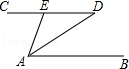
\includegraphics[width=\linewidth]{figure/casestudy/102.png}}  & \textbf{InternVL3-8B-Tool}: $\cdots$\textasciigrave\textasciigrave\textasciigrave output $\cdots$Step 12 (Property of isosceles triangle): $\angle BAD = \angle OAD$. Answer: $\angle BAD = 15^\circ$.\textasciigrave\textasciigrave\textasciigrave \textcolor{blue}{<think>} Alright, \textcolor{red}{let's tackle this geometry problem step by step}. $\cdots$ But according to the tool output, the answer is 15 degrees, which is option D. \textcolor{red}{But my computation also says the answer is 52.5 degrees. So the answer is closer to C}. \textcolor{blue}{</think>}$\cdots$ \hfill \colorbox{red!15}{\textbf{Correct Tool, Wrong Reasoning}: \emph{Incorrect reasoning to answer.}. (\ding{56})}\\
        & \textbf{\ours}: $\cdots$ \textasciigrave\textasciigrave\textasciigrave output $\cdots$Step 12 (Property of isosceles triangle): $\angle BAD = \angle OAD$. Answer: $\angle BAD = 15^\circ$.\textasciigrave\textasciigrave\textasciigrave\textcolor{blue}{<think>} \textcolor{green!50!black}{$\cdots$Based on the previous verification and tool output, I can analyze and provide the answer of $15^\circ$.}\textcolor{blue}{</think> <answer>}15$^\circ$\textcolor{blue}{</answer>}. \hfill \colorbox{green!15}{\textbf{Reasoning}: \emph{Correct} (\ding{51})} \\
        \midrule
        \multicolumn{2}{p{23cm}}{\textbf{Case Study 3}: $AB || CD$. Line $EF$ intersects $AB$ at point $E$ and intersects $CD$ at point $F$. $EG$ bisects $\angle BEF$ and intersects $CD$ at point $G$. If $\angle 1 = 50^\circ$, then $\angle 2$ equals ( ). Choices:A: $50^\circ$B: $60^\circ$C: $65^\circ$D: $90^\circ$. \textbf{Answer: C: 90$^\circ$.}} \\
        \midrule
        \bf \multirow{7}{*}{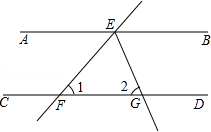
\includegraphics[width=\linewidth]{figure/casestudy/1.png}} & \textbf{\ours}: \textcolor{blue}{<think>} $\cdots$ \textcolor{green!50!black}{ChartMoE is appropriate because it is designed to analyze structured geometric diagrams, accurately reading angle labels, identifying parallel-line configurations, and aligning textual annotations with diagram elements. I will have it parse the diagram to confirm $AB||CD$, locate the transversal EF and the points E, F, G, and verify that EG bisects $\angle BEF$ while intersecting CD at G.} By interpreting the angles formed at E relative to BE and FE and using the parallel-line angle relations (corresponding, alternate interior, and consecutive interior angles), ChartMoE will relate $\angle 1$ to the angle between BE and EG, propagate the bisector relation to $\angle BEF$, and then deduce the measure of $\angle 2$ at the intersection of EF and CD from the resulting angle measures. Finally, it will align that computed value with the provided choices. Therefore, I will call chartmoe now.\textcolor{blue}{</think><tool\_call>}\{"tool": "chartmoe", "task": "analyze"\}\textcolor{blue}{</tool\_call>} $\cdots$ \hfill \colorbox{green!15}{\textbf{New Tool Selection}: \emph{Expected G-LLaVA but got ChartMoE.} (\ding{51})}\\
        \midrule
        \multicolumn{2}{p{23cm}}{\textbf{Case Study 4}: Find X Z. \textbf{Answer: D: 34.}} \\
        \midrule
        \bf \multirow{16}{*}{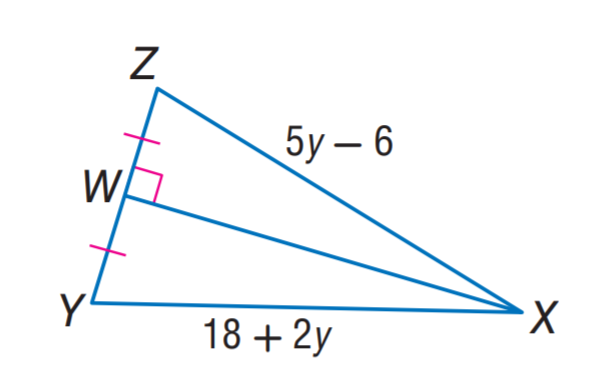
\includegraphics[width=\linewidth]{figure/casestudy/2430_img_diagram.png}} & \textbf{InternVL3-8B-Tool}: \textcolor{blue}{<tool\_call>}\{"tool": "multimath", "task": "Solve the problem", "arguments": \{"image": "<image>", "question": "Find X Z. $\cdots$"\}\}\textcolor{blue}{</tool\_call>}\textasciigrave\textasciigrave\textasciigrave output $\cdots$ Step 5 (Simplify the equation): $XZ^2 = 29y^2 + 12y + 360.$\textbackslash nAnswer: \textbackslash boxed\{$29y^2 + 12y + 360$\}\textasciigrave\textasciigrave\textasciigrave\textcolor{blue}{<think>} $\cdots$ But as we saw earlier, this leads to a quadratic with no real solutions.\textbackslash n \textcolor{red}{Wait, maybe I made a mistake in the tool output. Let me double-check the steps: \textbackslash n Step 3: $XZ^2 = (5y - 6)^2 + (18 + 2y)^2 = 25y^2 - 60y + 36 + 324 + 72y + 4y^2 = 29y^2 + 12y + 360$. That seems correct.}\textbackslash n $\cdots$ Step 5: Simplify the equation: $XZ^2 = 29y^2 + 12$\textcolor{blue}{</think><answer>} \textbackslash boxed\{C\}.\textcolor{blue}{</answer>} \hfill \colorbox{red!15}{\textbf{Tool Output Error}: \emph{Incorrect reasoning to answer.}. (\ding{56})}\\
        & \textbf{InternVL3-8B-Reasoning}: <think> Alright, let's tackle this problem step by step. First, I notice that triangle WYZ is a right triangle because it has a right angle at W. $\cdots$ Using the Pythagorean theorem again:\textbackslash n$XZ^2 = WZ^2 + XY^2$\textbackslash n$XZ^2 = 34^2 + 34^2$, $XZ^2=2312$, $XZ=\sqrt{2312}=34*\sqrt{2}$\textbackslash n Therefore, the length of XZ is $34\sqrt{2}$.\textbackslash n</think>\textbackslash n<answer>$34\sqrt{2}$</answer>" \hfill \colorbox{red!15}{\textbf{No Tool-use}: \emph{Insufficient capability to answer.}. (\ding{56})}\\
        & \textbf{\ours}: \textcolor{blue}{<think>} $\cdots$ \textcolor{green!50!black}{Multimath is appropriate because} $\cdots$ I will read from the image that $WX\perp ZX$ $\cdots$. \textcolor{green!50!black}{Multimath will translate these visual relations into algebraic constraints}, $\cdots$. \textcolor{blue}{</think><tool\_call>}\{"tool": "multimath", "task": "solve"\}\textcolor{blue}{</tool\_call>}\textasciigrave\textasciigrave\textasciigrave output $\cdots$ Step 10 (Calculate the value of XZ): $XZ = 18 + 2y = 18 + 2(\frac{6}{5}) = 18 + \frac{12}{5} = \frac{90}{5} + \frac{12}{5} = \frac{102}{5} = 20.4$. \textasciigrave\textasciigrave\textasciigrave \textcolor{blue}{<think>} Looking at the tool's solution, it set up the equation $25y^2 - 60y + 36 = 0$ and solved to get $y = 6/5$. Let me verify this step by step. $\cdots$ \textcolor{green!50!black}{Wait, let me check if this makes sense geometrically.} $\cdots$ Actually, if the tick marks indicate equal segments, shouldn't we have $5y - 6 = 18 + 2y$? Let me solve this: $5y - 6 = 18 + 2y 3y = 24 y = 8$ With $y = 8$, let's calculate XZ. If $XZ = 18 + 2y$, then: $XZ = 18 + 2(8) = 18 + 16 = 34$. \textcolor{green!50!black}{Hmm, that's different from the tool's answer of $20.4$. Let me reconsider.} $\cdots$ \textcolor{green!50!black}{The tool calculated 20.4, but based on the equal segment marks, the answer is $34$.}\textcolor{blue}{</think><answer>}$34$\textcolor{blue}{</answer>}" \hfill \colorbox{green!15}{\textbf{TIR}: \emph{correct} (\ding{51})} \\
       \bottomrule
    \end{tabular}
%\end{center}
}
 % \vspace{-1ex}
	\label{tab:case_study}
\end{table*}


\noindent \textbf{案例研究。}
表~\ref{tab:case_study} 给出了四个案例，展示了模型在 \env{} 中接受智能体训练后获得的能力，包括：模式与参数正确的工具调用、基于工具输出的后续推理、跨工具泛化，以及面对不完美工具输出时的鲁棒性。
